\usepackage[utf8]{inputenc}
\usepackage{graphicx}
\documentclass{beamer}
\usetheme{Antibes}
\usepackage{graphics}

\title{Predicción automática de palabras}
\author{Miguel Atencio, Andrés Cuervo}\textbf{Universidad del Rosario}
\date{Mayo de 2020}

\begin{document}

\maketitle

\begin{frame}{Tabla de contenidos}
    \begin{itemize}
        \item Introducción
        \item Descripción del Problema
        \item Marco Teórico
        \item Solución del problema
        \item Conclusiones
    \end{itemize}
\end{frame}

\begin{frame}{Introducción}
En este proyecto se desarrllo una herramienta de predicción de palabras, la cúal pretende ayudar a encontrar palabras que tengan sentido con el texto elegido.
\end{frame}

\begin{frame}{Descripción del problema}
El problema se basa en la predicción de palabras después de haber escrito al menos 
una palabra de referencia.Este problema tiene como necesidad una recolección de 
textos con los cuales posteriormente se espera predecir palabras en una oración con ayuda 
de los grafos.
    \begin{center}
        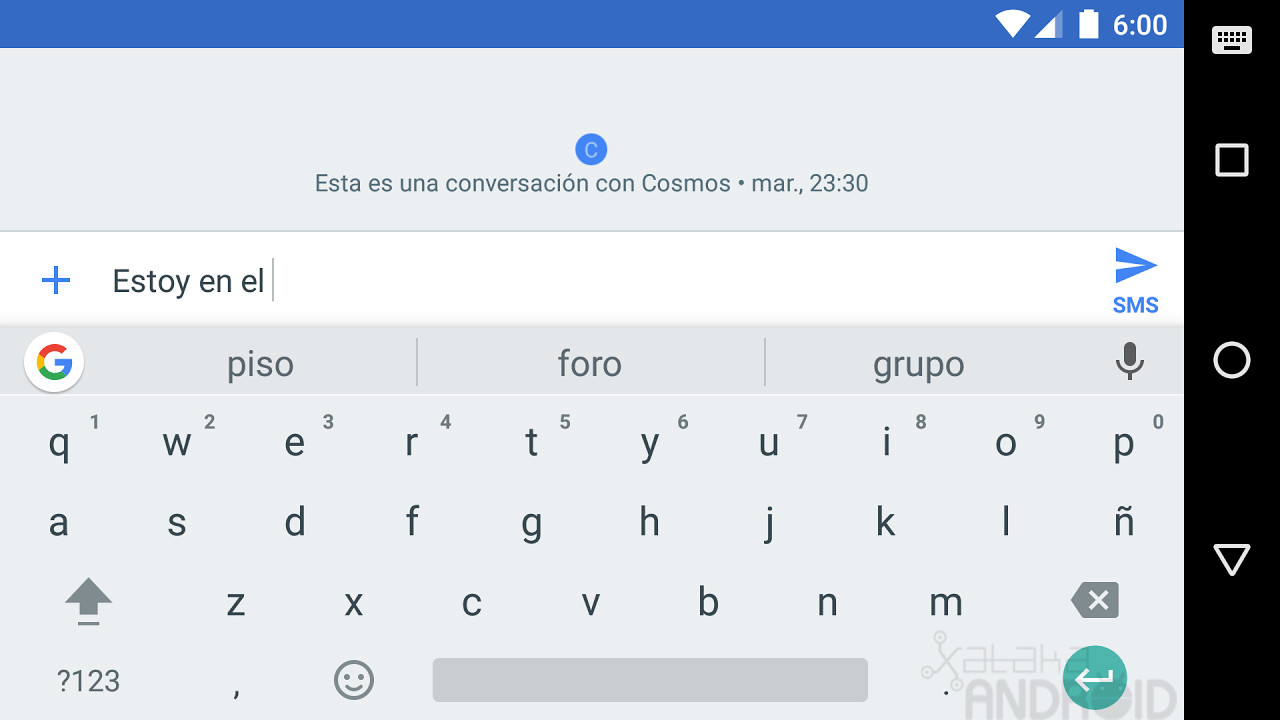
\includegraphics[width=.5\textwidth]{g0.jpg}
    \end{center}

\end{frame}

\begin{frame}{Marco Teórico}

    \begin{itemize}
        \item Grafos Dirigidos:
        Un grafo dirigido o digrafo G es una terna que consiste en un conjunto de vértices $V(G)$, un conjunto de aristas $E(G)$ y una función que asigna a cada arista un par ordenado de vértices.\\
        \begin{center}
            $f : E(G) \rightarrow V(G) \times V(G)$ \\
            $e \rightarrow f(e) = (u, v)$
        \end{center}
    \begin{center}
            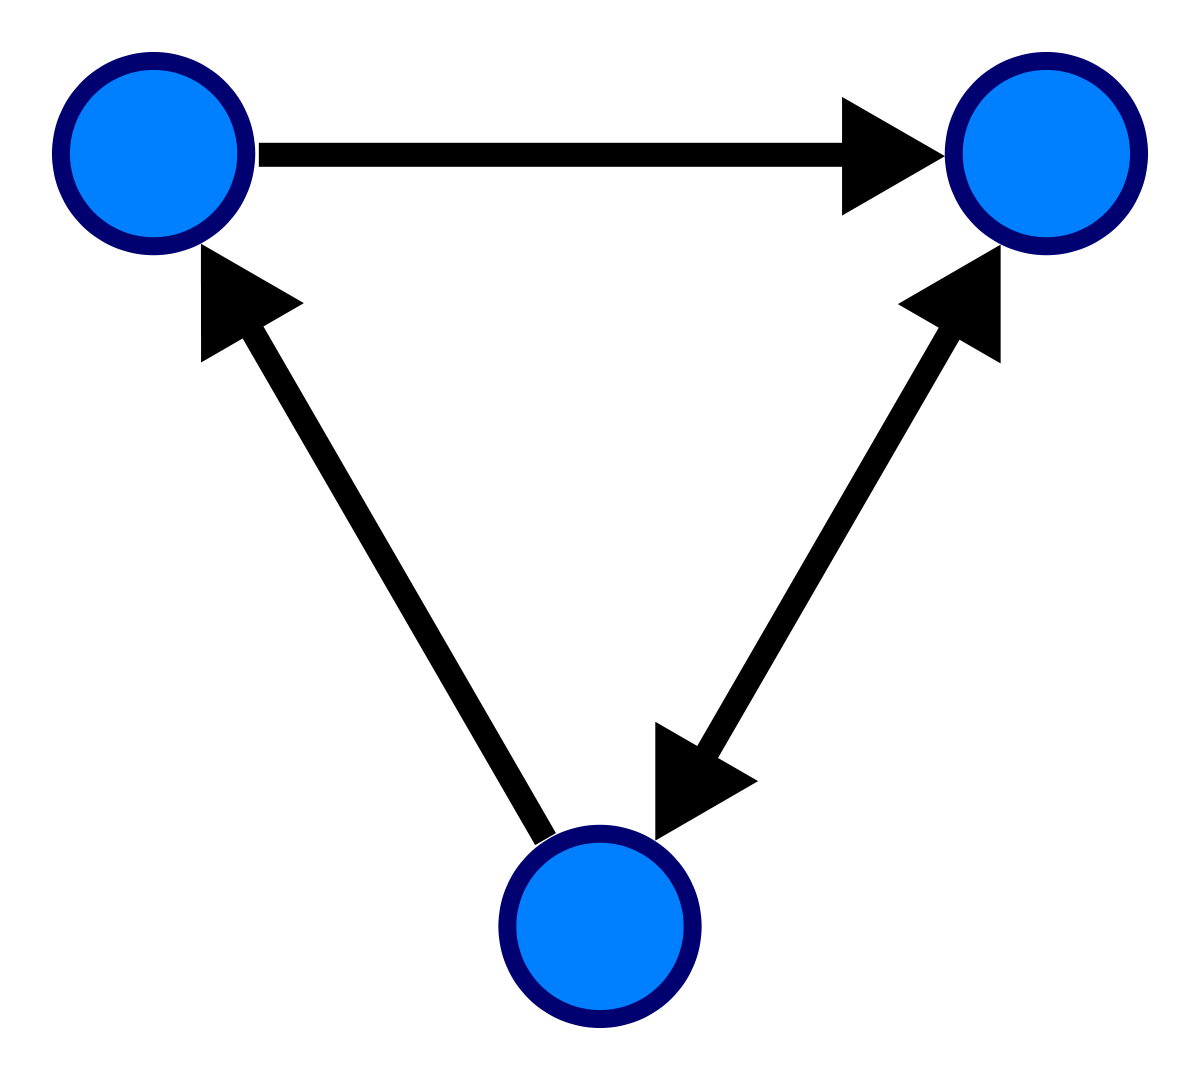
\includegraphics[width=.3\textwidth]{g1.png}
    \end{center}
    \end{itemize}

\end{frame}

\begin{frame}{Marco Teórico}
    \begin{itemize}
        \item Grafo Ponderado:
        Es un grafo con una asignación númerica en las aristas del grafo.
    \end{itemize}
    \begin{center}
        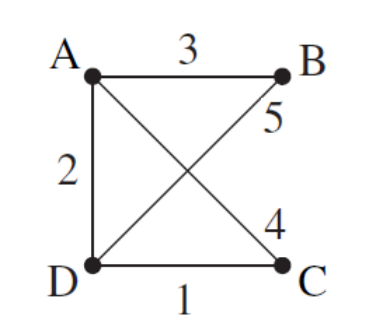
\includegraphics[width=.4\textwidth]{g2.png}
    \end{center}
\end{frame}

\begin{frame}{Solución del problema}
    Por medio de la recolección de textos creamos grafos dirigidos, en los cuales el vértice representa una palabra y la arista dirigida significa que palabra sigue después. Además, la cantidad de repeticiones de estas palabras representa el peso de la arista dirigida.
    
    \begin{center}
        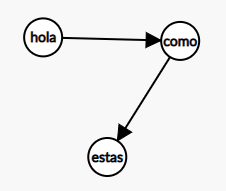
\includegraphics[width=.4\textwidth]{g3.png}
    \end{center}
    
\end{frame}

\begin{frame}{Conclusiones}
La tería de grafos desde el punto de vista computacional, aporta masivamente a las estructuras de datos y a la resolución de problemas computacionales, por lo que ha sido esencial para la herramienta creada.
Esta herramienta muestra como por medio de unos cuantos textos y con el algoritmo correcto, podemos predecir correctamente como algunas palabras están constituidadas para que al momento de crear oraciones esta tenga sentido.
\end{frame}

\begin{frame}{Referencias}

\begin{thebibliography}{3}
\bibitem{Douglas B. West}
\textit{Douglas B. West Introduction to graph theory, 2nd edition.2000.}

\bibitem{}
Bojacá, Daniel.
\textit{Grafos dirigidos [Material de clase]}
Universidad del Rosario, Bogotá D.C. 2020

\bibitem{}
Bojacá, Daniel.
\textit{Árboles - Aplicaciones [Material de clase]}
Universidad del Rosario, Bogotá D.C. 2020

\end{thebibliography}
    
\end{frame}
\end{document}


